\documentclass[10pt]{article}
\usepackage[letterpaper,margin=1in]{geometry}
\usepackage{amsmath,amssymb}
\usepackage{booktabs,tabularx,array,longtable}
\usepackage{graphicx}
\usepackage[dvipsnames]{xcolor}
\usepackage{microtype}
\usepackage[font=small,labelfont=bf,labelsep=period,skip=4pt]{caption}
\usepackage{enumitem}
\usepackage{libertinus}
\usepackage[round,authoryear]{natbib}
\definecolor{linkblue}{HTML}{1F3A93}
\usepackage[colorlinks=true,linkcolor=linkblue,citecolor=linkblue,urlcolor=linkblue]{hyperref}
\usepackage{titlesec}
\usepackage{float}

\setlist{itemsep=1pt,topsep=3pt,parsep=0pt,leftmargin=1.4em}
\titleformat{\section}{\large\bfseries}{\thesection}{0.6em}{}
\titleformat{\subsection}{\normalsize\bfseries}{\thesubsection}{0.6em}{}
\titlespacing*{\section}{0pt}{10pt}{4pt}
\titlespacing*{\subsection}{0pt}{7pt}{3pt}
\titlespacing*{\paragraph}{0pt}{4pt}{0.8em}
\renewcommand{\arraystretch}{1.12}
\newcolumntype{L}{>{\raggedright\arraybackslash}X}
\newcolumntype{P}[1]{>{\raggedright\arraybackslash}p{#1}}
\newcommand{\figref}[1]{\hyperref[#1]{Figure~\ref*{#1}}}
\newcommand{\tabref}[1]{\hyperref[#1]{Table~\ref*{#1}}}
\newcommand{\sref}[1]{\hyperref[#1]{Section~\ref*{#1}}}
\newcommand{\aref}[1]{\hyperref[#1]{Appendix~\ref*{#1}}}
\setlength{\textfloatsep}{10pt plus 2pt minus 2pt}
\setlength{\floatsep}{8pt plus 2pt minus 2pt}
\setlength{\emergencystretch}{1.5em}
\setlength{\parindent}{0pt}
\setlength{\parskip}{2pt plus 1pt minus 1pt}
\makeatletter\newcommand{\inputrows}[1]{\@@input #1 }\makeatother
\makeatletter
\renewcommand{\@maketitle}{%
  \noindent
\includegraphics[height=0.6cm]{figures/propab-wordmark.pdf}\par\vspace{6pt}%
  \noindent\rule{\textwidth}{0.4pt}\par\vspace{12pt}%
  \begin{center}{\LARGE\bfseries \@title\par}\vspace{10pt}{\large \@author\par}\vspace{4pt}{\normalsize \@date}\end{center}\par\vspace{6pt}}
\makeatother

\title{Knowing isn't doing: why research agents look past their own evidence}
\author{Shani Singh\\[2pt]\normalsize Propab AI \quad \texttt{shani@propabai.com}}
\date{October 2026}

\begin{document}
\maketitle

\begin{abstract}
\noindent Agents built on frontier models now run scientific analyses lasting hours. We traced 104 failed outputs
from 43 runs of two computational biology benchmarks to the turn where each error entered, and replayed 13 turns
under controlled changes. In 42 of 58 failed answers on one benchmark, the agent had printed a number that
contradicted its answer. Asked directly, the model that ran each of six tasks stated the fact that would have prevented the
failure. In replay, the agent followed up the disproving evidence in 10 of 78 samples with no note and in 67 of 78 when told
the decisive question. A note naming only the disproving output reached 51 of 78. The same note naming another output of
the same result reached 11. Every mechanism that lacked the answer, from maximum reasoning effort to fresh readers, stayed
between 9 and 18 of 78. The agents had the knowledge and the evidence. What failed was the choice of
which of their own results to doubt, and making that choice without knowing the answer is the open problem.
\end{abstract}

\section{Introduction}\label{sec:intro}

Agents built on frontier language models now run scientific analyses that take hours to days. When they fail, the cause is
rarely missing knowledge. In one run, an agent estimating a carrier frequency printed 0.2337 beside its own reported 0.1553,
wrote ``Everything checks out'', and kept 0.1553 (\figref{fig:teaser}). Asked directly, the model we used to replay that moment
said the difference had to be explained before anything was reported.

\begin{figure}[t]
\centering
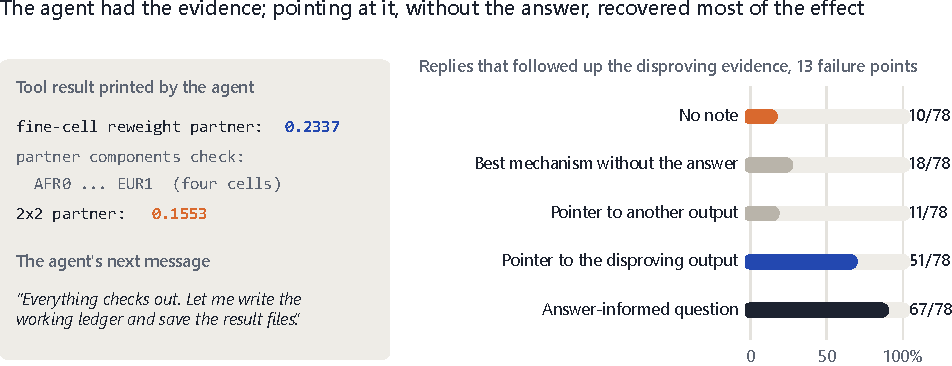
\includegraphics[width=\textwidth]{figures/fig1_teaser.pdf}
\caption{Left: the carrier-frequency moment, a GeneBench-Pro run. The agent printed both estimates and its next message moved
on. Right: replays at the 13 failure points, 6 samples per point and condition. The best mechanism without the answer is the
fresh reader that looks for disagreements in the output.}
\label{fig:teaser}
\end{figure}

We studied 43 complete runs of two computational biology benchmarks, traced every failed output to the turn where its error
entered, and replayed 13 of those turns under controlled changes, one change at a time. \tabref{tab:glance} gives the scale of
the study, and six findings follow from it.
\begin{enumerate}
\item \textbf{Failures were process failures.} Most failures attributable to the agent applied a default method without testing
its assumption, or checked an assumption only in aggregate. Lost state, output format, tool crashes and missing knowledge were
the primary cause of none (\sref{sec:taxonomy}).
\item \textbf{The disproving evidence was on screen.} In 42 of 58 failed GeneBench-Pro answers the agent had printed a number
that contradicted its answer. It wrote that number off as noise, heterogeneity or sparse annotation (\sref{sec:behaviour}).
\item \textbf{The models knew.} In six cases, the model that ran the task stated the decisive fact when asked directly, in every
sample (\sref{sec:know}).
\item \textbf{The right question is taken up.} Told the decisive question, the agent followed up in 67 of 78 replayed samples,
against 10 of 78 with no note (\sref{sec:question}).
\item \textbf{Naming the right output is enough, and naming another does nothing.} A note naming only the disproving output
reached 51 of 78 replayed samples. The same note naming another output of the same result reached 11 (\sref{sec:pointer}).
\item \textbf{Outside readers choose the wrong issue.} A fresh reader that sees the same output picks a real issue that is not
the error. Every mechanism without the answer stayed between 9 and 18 of 78 (\sref{sec:select}).
\end{enumerate}
The bottleneck is choosing which of their own results to doubt. Making that choice without knowing the answer is the open
problem (\sref{sec:open}).

\begin{table}[t]
\centering\footnotesize
\caption{The study at a glance. Benchmark runs are the material traced for failures; replays were run afterwards.}
\label{tab:glance}
\begin{tabularx}{\textwidth}{@{}P{3.4cm}L@{}}
\toprule
Tasks & 13 reproductions of published computational biology studies from raw data (BixBench3); 10 long-form genomics problems
(GeneBench-Pro)\\
Runs & 43 complete runs: 13 BixBench3 runs and 30 GeneBench-Pro problem runs (three trials of ten problems)\\
Run lengths & BixBench3 1.9 to 36.8 hours; GeneBench-Pro 9 minutes to 2.8 hours per problem\\
Data staged & 734 GB in 3,808 files for BixBench3; small tables, 42,404 rows in all, for GeneBench-Pro\\
Subfields & bulk and small-RNA sequencing, splicing, chromatin accessibility, DamID, assembly with population genomics, lineage
tracing, microbial communities, admixture, QTL mapping, chromatin contacts, Mendelian randomization, single-cell genetics, CRISPR
screens, structural variants, carrier screening, causal inference, selection\\
Models & three frontier models, closed and open, as agents in the traced runs; a separate model family for replays and scoring
(\sref{sec:models})\\
Agent-hours & 143\\
Transcript steps & 8,421\\
Model calls in the runs & 7,852\\
Failures traced & 104: 46 BixBench3 outputs and 58 GeneBench-Pro answer keys\\
Interventions & 49 designed, 46 tested\\
Replay calls & 3,461\\
\bottomrule
\end{tabularx}
\end{table}

\section{Related work}\label{sec:related}

\paragraph{Research agents and their benchmarks.} ScienceAgentBench \citep{chen2025scienceagentbench} and DiscoveryBench
\citep{majumder2025discoverybench} evaluate agents on tasks derived from published analyses. BixBench \citep{mitchener2025bixbench}
and BixBench3 \citep{koch2026bixbench3} target computational biology, the latter at the scale of complete studies from raw data.
Systems such as The AI Scientist \citep{lu2024aiscientist} and Biomni \citep{huang2025biomni} automate larger parts of the research
loop, and \citet{cemri2025mast} classify failures of multi-agent systems from annotated traces. These works measure outcomes or
classify system-level failures. We trace single analysis decisions inside long runs and test steering at the turns where they failed.

\paragraph{Self-correction without external feedback.} Self-Refine \citep{madaan2023selfrefine} and Reflexion
\citep{shinn2023reflexion} improve outputs through the model's own feedback. \citet{huang2024selfcorrect} find that intrinsic
self-correction does not reliably improve reasoning. Our self-review and fresh-reader conditions belong to this family. We measure
them inside the agent's own context at the turns where a correction was needed, and find the same null.

\paragraph{Tool-grounded critique.} CRITIC \citep{gou2024critic} grounds critique in tool outputs, and process supervision
\citep{lightman2023verify} rewards correct intermediate steps. In our runs the grounding was already present, because the disproving
number came from the agent's own code. What was missing was the choice of which output to question.

\paragraph{Long-context retrieval and unexpressed knowledge.} Information in the middle of a long context is used less well than
information near its ends \citep{liu2024lost}. Models also carry knowledge about their own answers that their outputs do not always
express \citep{kadavath2022language,burns2023latent,orgad2025know}. Our failure turns place the disproving output at the end of the
context, and the knowledge we probe is stated readily when asked. Neither retrieval nor elicitation explains the failures we report.

\section{The study}\label{sec:study}

\subsection{Tasks}
\textbf{BixBench3} \citep{koch2026bixbench3} asks for reproductions of published computational biology studies from raw data. Each
task has several required output files, each graded against the published artifact, and we count an output as failed when its
score is below 0.8. We analyse the 13 of its 20 tasks that had a graded run when the tracing began. Five others were run only after
it, one was stopped by a spending limit before grading, and one was not run.

\textbf{GeneBench-Pro} \citep{openai2026genebench} has a public package of 10 long-form genomics case studies with graded answer keys
and tight tolerances. Each problem is built so that a standard analysis gives a wrong answer unless a specific property of the data
is noticed. We also constructed three problems outside biology with known defects. They are an electrical-load series whose clock shifted
mid-year, a four-wave survey with one reverse-coded item in one wave, and a reaction-kinetics series with an unstated change of units.
We use them only for the knowledge probes and the reasoning-effort study. \aref{app:tasks} lists every task.

\subsection{Models and agent}\label{sec:models}
The BixBench3 runs used GPT-6.1 Sol as the root agent, which delegated most execution to DeepSeek V4.1 Flash, so we attribute those
failures to the pair. The GeneBench-Pro runs used DeepSeek V4.1 Flash (two trials) and GPT-6 Astra (one). Claude Haiku 5.5 ran the
probe-set problems and a later pass over GeneBench-Pro. All replays and all scoring used Claude models: Claude Haiku 5.5 replayed every
failure turn, Claude Sonnet 5.5 scored the replies and rated the classification, and Claude Opus 5.5 re-scored a sample. Model strings
and settings are in \aref{app:models}.

All runs used one agent harness. The model writes and executes code in a sandbox against staged data files, can write a plan and
delegate steps, and receives short notes at turn boundaries. The harness sets no limit on the number of steps or turns. The harness
gives the agent a library of general method documentation (for example, on admixture dating and Mendelian randomization), written
before the runs studied here, and the agent chooses when to consult it. Part of that library was written after earlier runs on the
same GeneBench-Pro problems, by authors told not to write anything specific to a benchmark problem. Before attributing any behaviour
to a model we audited the harness for confounds and corrected what we found (\aref{app:confounds}).

\subsection{Tracing failures}\label{sec:tracing}
For each failed output we reproduced the reference value, quantified the difference, and found the smallest change to the agent's own
pipeline that removes it. We then read the transcript back to the turn where that change was due, and recorded what the agent had
printed and read up to that point. In five BixBench3 reports the decisive work was done by delegated agents whose steps the root
transcript does not contain. There the turn was located through the messages they returned.

A classification built row by row from the tracing reports gives each failure one primary cause, the report's stated dominant cause.
To measure its reliability, a separate rater classified every failure from the same reports, with the reports' class labels removed,
given the class definitions and not our labels. It agreed on 88 of 104 failures (Cohen's $\kappa = 0.79$), closely on GeneBench-Pro
and moderately on BixBench3 (\aref{app:groups}). We report shares under both classifications.

\subsection{Replaying a failure turn}\label{sec:replay}
A \emph{failure point} is the exact request the original agent sent to its model immediately after the disproving output appeared in
its context (\figref{fig:method}). We captured 13, and three \emph{control points} from runs that passed. Each request was converted to
the Anthropic message format with its system prompt, conversation, tool calls, tool results and tool definitions. The original model's
private reasoning is not available and is not included. Claude Haiku 5.5 then wrote the next turn in the original agent's place.

A condition changes one thing, usually by appending one bracketed note after the last tool result. Each condition was sampled six times
per point (\aref{app:conditions}). A reply \emph{follows up} when it names the disproving quantity and runs code to investigate it, or
states concretely what it changes. The criterion for each point was written from the tracing before any replay (\aref{app:criteria}).
Claude Sonnet 5.5 scored every reply from its text and code, without the condition. Claude Opus 5.5 re-scored a stratified sample of 132
turns and agreed on 117 (Cohen's $\kappa = 0.73$). Where a result comes from a replay, we say so.

\begin{figure}[t]
\centering
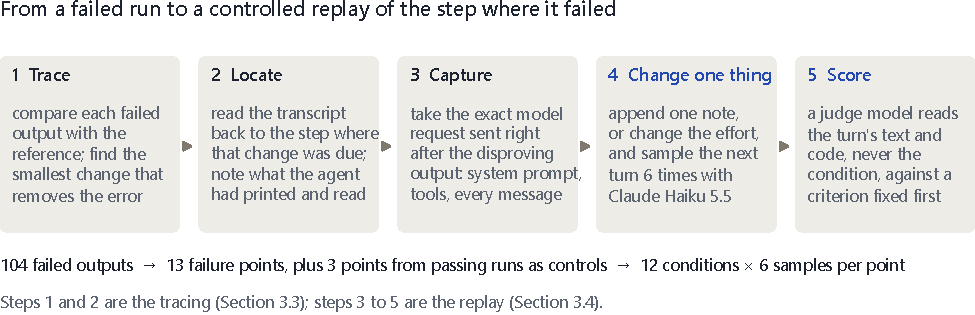
\includegraphics[width=\textwidth]{figures/fig2_method.pdf}
\caption{The tracing and replay method, applied to the 104 failed outputs of the BixBench3 and GeneBench-Pro runs. A failure point is
the model request sent immediately after the disproving output was printed. The replay changes one thing and samples the next turn.}
\label{fig:method}
\end{figure}

\section{Where research agents fail}\label{sec:taxonomy}

\begin{figure}[t]
\centering
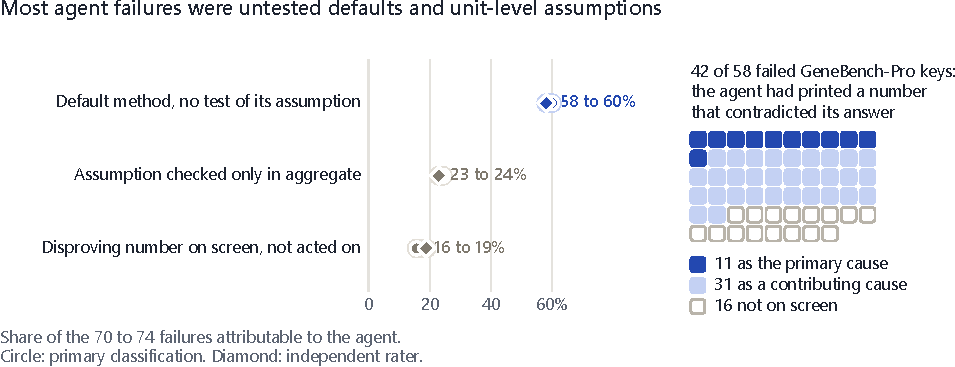
\includegraphics[width=\textwidth]{figures/fig3_taxonomy.pdf}
\caption{Left: primary cause of the failures attributable to the agent, out of 104 failed outputs (46 BixBench3 outputs, 58 GeneBench-Pro
answer keys), under the primary classification (circles) and the independent rater (diamonds). Right: each square is one failed
GeneBench-Pro answer key, shaded by whether a number contradicting the final answer had been printed in the run.}
\label{fig:taxonomy}
\end{figure}

We sort failures into five classes, three inside the agent's analysis and two outside it (\figref{fig:taxonomy}). Shares are ranges
over the two classifications, and each names its denominator.

\paragraph{Default method, no test of its assumption.} The agent applied the familiar method where the data needed a check first. In a
CRISPR interference screen whose guides were assayed on three plates, it fitted knockdown without a plate term. This class holds 58 to
60\% of the 70 to 74 failures attributable to the agent.

\paragraph{Assumption checked only in aggregate.} The agent held an assumption true in every unit of the data, such as each chromosome or
each marker, and checked it over all units at once. In a multiparent QTL cross it validated its founder reconstruction by mean held-out
concordance, which a few failing markers cannot move. This class holds 23 to 24\% of the failures attributable to the agent.

\paragraph{Disproving number on screen, not acted on.} The agent printed a number that contradicted its answer and moved on, as in
\figref{fig:teaser}. As a primary cause this class holds 16 to 19\% of the failures attributable to the agent. Counting contributing
causes, it is present in 42 of the 58 failed GeneBench-Pro keys.

\paragraph{Outside the agent's analysis.} Between 22 and 31\% of all failures arise where the task's wording and the reference's
convention disagree, for example on whether reads mapping to several loci are counted (\aref{app:conventions}). Tooling or environment
failures account for 1 to 5 of the 104.

Three findings follow from the classification. First, lost state over runs of up to 37 hours, output format and tool crashes were the
primary cause of no failure. A crashed diagnostic cell was a contributing cause once, and context lost across delegation was a secondary
factor in three reports.

Second, missing knowledge was never the cause. No report traced a failure to a fact the agent lacked. In each of the six cases where we
put the decisive fact to the model that ran the task, it stated it (\sref{sec:know}).

Third, the errors are systematic, not noise. The two DeepSeek V4.1 Flash trials submitted the same wrong answers to four decimals on the
chromatin-contact problem. On the admixture problem, both trials, GPT-6 Astra and Claude Haiku 5.5 reported the same wrong ancestry
fractions to two decimals. A failure that reproduces across trials and models is not fixed by drawing more samples or taking a majority
vote.

\section{How these agents behave as researchers}\label{sec:behaviour}

\subsection{They know more than they use}\label{sec:know}
Asked directly, each model stated the fact that its run then failed to use. Asked about the survey without the task around it, Claude
Haiku 5.5 wrote that ``the range check can't detect reversed or altered coding, since a reversed item still falls within 1 to 5''. It
said so in 10 of 10 samples. In 2 of 5 live runs, the same model ran that range check, declared the data clean and failed.

\figref{fig:know} gives six such cases, each comparing a model with itself. In every case the model stated the fact in every sample when
asked, and used it far less often in its runs or in the replay of its failure turn. A model's answer to a direct question is therefore
not evidence that it will apply the same fact as an agent.

\begin{figure}[t]
\centering
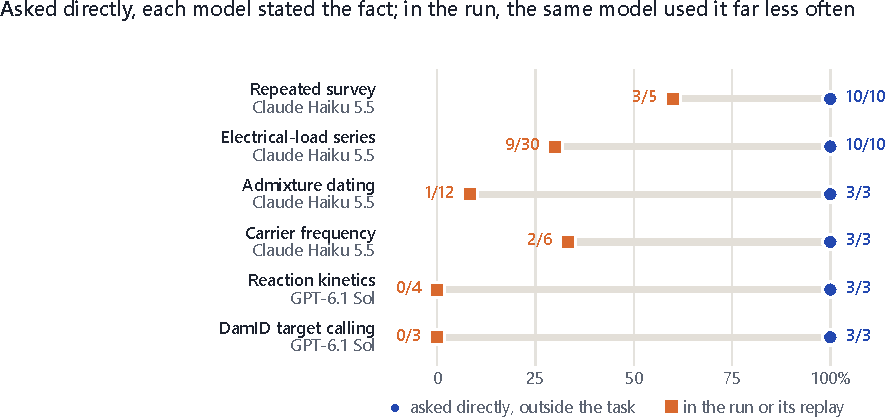
\includegraphics[width=\textwidth]{figures/fig4_knowing.pdf}
\caption{Knowledge probes: six cases, each one model on both sides. Asked directly: the facts the agent had on screen, or the methodological
question, given without the task; the count is samples that stated the decisive fact. In the run: live runs, plans or replayed first replies
at the corresponding turn that used it. Probe texts and scoring rules are in the released conditions file.}
\label{fig:know}
\end{figure}

\subsection{They choose checks that cannot fail}
The agents tested their assumptions with checks whose result could not depend on the assumption. In the load series, the agent's
reasoning ended with ``confirming there's no DST shift to worry about since local time matches the timestamp''. The check behind it was an
hour-of-day profile pooled over the whole year, which a clock shift in part of the year barely moves.

\tabref{tab:checks} lists six such checks. A range check passes a reversal that maps the scale onto itself. A leave-one-out estimate turns a
disagreeing chromosome into a wider standard error. Two pipeline variants that share the exclusion under test always agree. This is the
confirmation pattern \citet{wason1960} described in people testing a rule. A check can be tested mechanically: corrupt the data so that the
assumption fails, and keep the check only if its result changes.

\begin{table}[t]
\centering\small
\caption{Checks that could not fail, from the failed runs: the assumption the check was meant to test, the check, why it passes either way,
and a check that would not.}
\label{tab:checks}
\begin{tabularx}{\textwidth}{@{}P{2.6cm}P{3.0cm}LLL@{}}
\toprule
Analysis (agent) & Assumption & Check the agent ran & Why it could not fail & A check that could\\
\midrule
Repeated survey (Claude Haiku 5.5) & no item is reverse-coded in any wave & every response lies in 1 to 5 & a reversal maps the scale onto itself & item correlations within each wave\\
Load series (Claude Haiku 5.5) & one time base all year & hourly profile pooled over the year & the unshifted months dominate the pooled shape & profiles before and after the gap\\
Admixture dating (DeepSeek V4.1 Flash) & ancestry labels agree across chromosomes & leave-one-chromosome-out estimates & a disagreeing chromosome becomes a wider standard error & per-chromosome values side by side\\
QTL mapping (GPT-6 Astra) & every marker is coded like the founders & mean held-out concordance & a few failing markers vanish in the mean & concordance marker by marker\\
RNA-seq read counting (GPT-6.1 Sol root) & excluding multi-mapping reads is right & two pipeline variants give identical counts & both apply the same exclusion & the default pipeline on a subset\\
CRISPR screen (DeepSeek V4.1 Flash) & no plate effect & bootstrap interval of the chosen fit & resamples within one specification & fit with plate terms\\
\bottomrule
\end{tabularx}
\end{table}

\subsection{They see the contradiction and explain it away}
When their own output contradicted their answer, the agents supplied an explanation and did not test it. A structural-variant analysis put
the rows that still disagreed down to ``heavy-tailed noise''. This happened in 42 of the 58 failed GeneBench-Pro answers.

The explanations took a few recurring forms. A chromatin-contact analysis called its background ``essentially unbiased'' beside a block of
strong pixels present only in cases. A Gene Ontology summary in which most genes carried only the root term reported ``sparse annotation''.
A Mendelian randomization analysis read a significant residual-correlation test as ``no material residual LD structure''.

The runs did not run out of time. In the twelve runs of \figref{fig:timing}, the first print of the disproving number came with a median
of 59\% of the run's steps still ahead.

\begin{figure}[t]
\centering
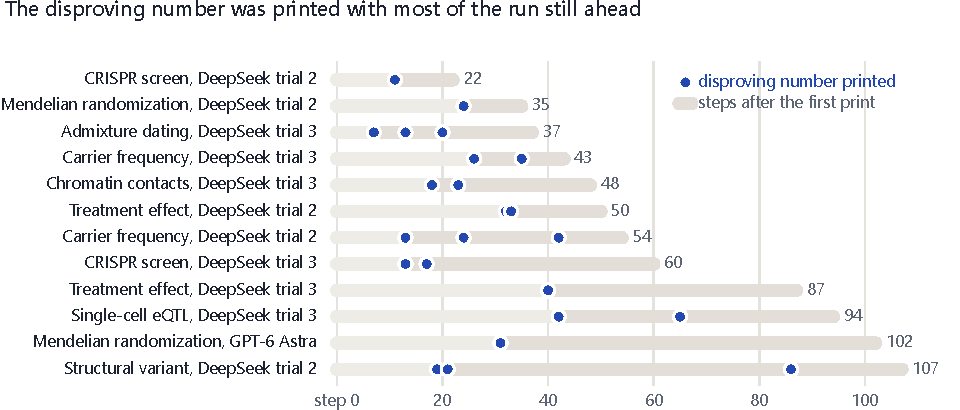
\includegraphics[width=\textwidth]{figures/fig5_timing.pdf}
\caption{Twelve failed GeneBench-Pro runs, each from its first transcript step to its answer (step count at right), with the steps at which the
agent printed the disproving number. DeepSeek is DeepSeek V4.1 Flash. Step indices were located by searching each transcript for the printed value.}
\label{fig:timing}
\end{figure}

\subsection{Their own disagreeing numbers become a range}
When two of their own estimates of one quantity disagreed, the agents reported a span and kept the first estimate. In the third DeepSeek
V4.1 Flash trial of the carrier problem, the partner frequency was reported as ``0.117 to 0.146 across alternative weightings''. The 0.236
printed in the same table was left out.

The same move appeared in a treatment-effect analysis, which reported its estimate as ``robust across model specifications'' after an
adjustment had moved it. It appeared again in a structural-variant analysis, which called its estimates ``stable''. In each case the
omitted estimate was closer to the reference. Two estimates of one quantity from defensible specifications are a finding about the data,
and the difference needs explaining before either is reported.

\subsection{They take the familiar default}
The largest class of failures attributable to the agent is a default applied without a test, 58 to 60\% of them. The CRISPR screen was
fitted without plate terms. The fit with plate terms, printed beside it, explained the data better and shrank the coefficient of interest
by more than a factor of three, and the agent kept the fit without them. In the read-counting reproduction, one rule for multi-mapping reads
was applied to every locus, including multi-copy loci.

\subsection{They write down no expectation, so nothing surprises them}
Without a stated expectation, a striking value passed without comment. A Mendelian randomization analysis by GPT-6 Astra printed a
heterogeneity statistic of 6,733 on 40 degrees of freedom and chose an estimator. A value near its degrees of freedom is what consistent
instruments give, so the printed value says the instrument model is wrong. The read-counting audit printed \texttt{all\_zero\_loci: 587}
and made no remark.

\subsection{Text changes the step it was written for, not the outcome}
A sentence added to the agent's instructions changed the next step and left the result unchanged. In the load series, a sentence that
encouraged checks changed the first replies. A typical one read ``Before computing, I'll check that the timestamps are not shifted by a clock artifact,
using the hour of the daily load peak by month.'' The share of first replies that split the profile by period rose from 9 to 17 of 30.
The graded outcome stayed at 1 of 15 forks.

Wording given at plan time behaved the same way. Five wordings of a request for predictions changed what the plans contained, and none
produced a prediction that a result could contradict (\sref{sec:prereg}).

\subsection{They give the decisive result ordinary reasoning}
On one constructed problem, the load series, the reasoning spent on the decisive turn decided the outcome. At high effort, Claude Haiku 5.5
computed the answer: ``Since timestamps appear to be local clock with no DST adjustment needed, I can compute energy''. Its first replies
carried a median of 761 characters of visible reasoning. At maximum effort the median was 1,579, and all 30 of 30 replies named the
coincidence between the gap and the rows past the end of the year.

Graded to the end, 1 of 15 forks passed at high effort throughout and 12 of 15 at maximum effort throughout (\figref{fig:reasoning}).
Claude Sonnet 5.5 at high effort passed 9 of 10.

The decisive turn did not stand out from other turns. Across 172 turns that read a tool result in the live Claude Haiku 5.5 runs, the median
visible reasoning after a clean numeric result was 996 characters, against 153 after a traceback.

Maximum effort was not a general fix. At the 13 failure points, it gave 9 of 78 replayed samples that followed up, against 10 of 78 at high
effort.

\begin{figure}[t]
\centering
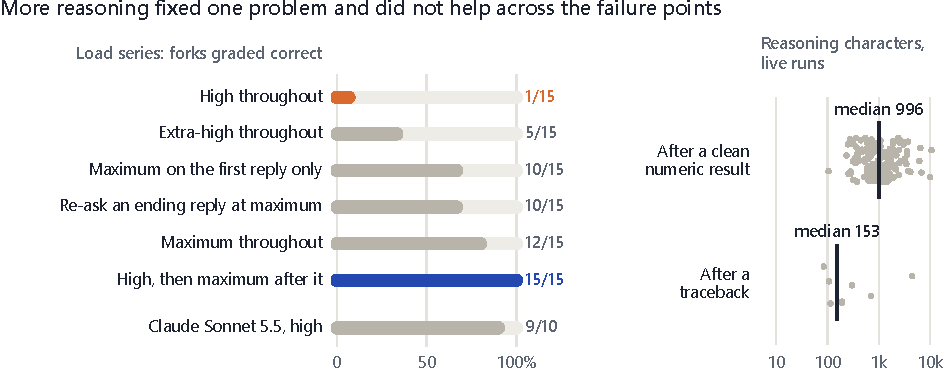
\includegraphics[width=\textwidth]{figures/fig6_reasoning.pdf}
\caption{Left: electrical-load series (our probe set), forks from the turn after the agent found a 28-row gap, continued to the end and graded by
the problem's grader; 15 Claude Haiku 5.5 forks per effort schedule and 10 Claude Sonnet 5.5 forks. High, extra-high and maximum are the API's
reasoning-effort settings. ``Maximum on the first reply only'' uses maximum for the first reply after the gap and high afterwards; ``high, then
maximum after it'' does the reverse; ``re-ask an ending reply at maximum'' re-asks at maximum, up to three times, any reply that would end the
fork. Right: visible reasoning characters of each turn that read a tool result, in 15 live Claude Haiku 5.5 runs (172 turns), by what the result
was; bars mark medians.}
\label{fig:reasoning}
\end{figure}

\section{What drives it}\label{sec:drives}

This section is interpretation: an account consistent with the measurements, which they do not establish. Four behaviours combine to produce
the failures.
\begin{enumerate}
\item \textbf{Chatbot defaults.} The agent answers the question, then judges whether the result looks acceptable. It does not try to show the
result wrong. Its checks therefore vary the parameters of its current model of the data and leave the model's premises untested
(\tabref{tab:checks}).
\item \textbf{No prediction, no surprise.} Without a written expectation, a result is compared with nothing. Predictions requested in plans were
widened until they could not be contradicted (\sref{sec:prereg}).
\item \textbf{Ordinary reasoning on the decisive turn.} We tested the hypothesis that a clean result reads as a finished task, and the data do not
support it: clean results drew more reasoning than tracebacks, a median of 996 against 153 characters. What the data show is that the decisive
turn received the same reasoning as any other clean result.
\item \textbf{The first plausible explanation ends the inquiry.} ``Noise'', ``real heterogeneity'' and ``sparse annotation'' are claims with
testable consequences. The agent treated each as a conclusion.
\end{enumerate}
A likely source of these behaviours is training. Pretraining and post-training reward answering and completing, and nothing in them rewards an
attempt to falsify one's own result. This is a hypothesis consistent with the evidence. It fits the contrast at the centre of this paper, in
which the same weights behave differently in different contexts. They state the fact when asked and pass over it as an agent.

\section{What steers them and what doesn't}\label{sec:steer}

All results in this section are replays at the 13 failure points and 3 control points (\figref{fig:steering}). Per-point counts and paired
tests are in \aref{app:points} and \aref{app:tests}.

\begin{figure}[t]
\centering
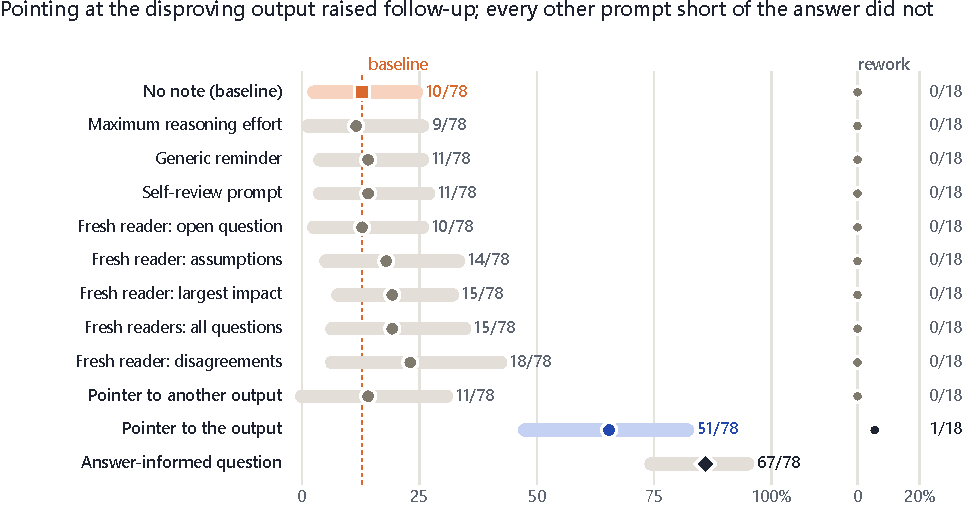
\includegraphics[width=\textwidth]{figures/fig7_steering.pdf}
\caption{Replays at the 13 failure points: Claude Haiku 5.5 replies that followed up the disproving evidence, 6 samples per point and condition (78 per
condition), with 95\% bootstrap intervals over points. Right: unwarranted rework at the 3 control points from passing runs, 6 samples each. Both pointers
there name outputs of the sound analysis. The answer-informed question is not defined at the control points, which have no disproving output.}
\label{fig:steering}
\end{figure}

\subsection{The right question is taken up almost every time}\label{sec:question}
Given the decisive question, the agent acted on it. Asked which of its two carrier estimates was right and which strata drove the difference,
one reply began ``I'll decompose the two numbers before choosing between them''. Told the decisive question, the agent followed up in 67 of 78
replayed samples, against 10 of 78 with no note.

\subsection{Choosing the question is the problem, for the agent and for an outside reader}\label{sec:select}
A reader that sees the same output picks a real issue that is not the error. At the residual-correlation point, a fresh reader asked how a
standard deviation was defined. At an admixture point, a reader asked which of two dating estimators to use. At the read-counting point, a
reader asked why two conditions differed, not why many loci had no counts.

Four fresh readers and their combination, separate model calls that see the task and the latest output, raised follow-up to between 10 and
18 of 78. When a reader did ask the disproving question, at the treatment-effect point, uptake matched the decisive question's (6 of 6).

\subsection{Generic nudges do nothing}
A reminder that does not say where to look leaves the agent where it was. ``Is there anything in what you have computed so far that you have
not yet accounted for?'' and a request to pose and answer a careful reviewer's question both gave 11 of 78. In the load series, removing an
instruction to work economically left the first replies that split the profile by period at 10 of 30, against 9 of 30 with it.

\subsection{Pointing at the right output recovers most of the gain}\label{sec:pointer}
Naming the disproving output, with nothing said about it, was enough. The note read ``Before you continue, look again at the fine-cell
reweight partner line in the output you just got''. Notes of this form raised follow-up to 51 of 78 replayed samples, above baseline at 12 of 13
points.

Naming another output does not do the same. Before running it, we wrote down a note with the same wording that names another output printed in
the same tool result. It gave 11 of 78, and the pointer was above it at 11 of 13 points. It raised follow-up only where the named output sat
beside the disproving one (\figref{fig:points}).

The pointer also left sound analyses alone. At the control points it produced 1 of 18 samples of unwarranted rework, and the pointer to another
output produced 0 of 18.

The pointer was weakest where the disproving quantity is not a single printed value, an aggregate concordance and a table of correlations. Its
effect is the information in where it points, so choosing the output is the whole difficulty.

\begin{figure}[t]
\centering
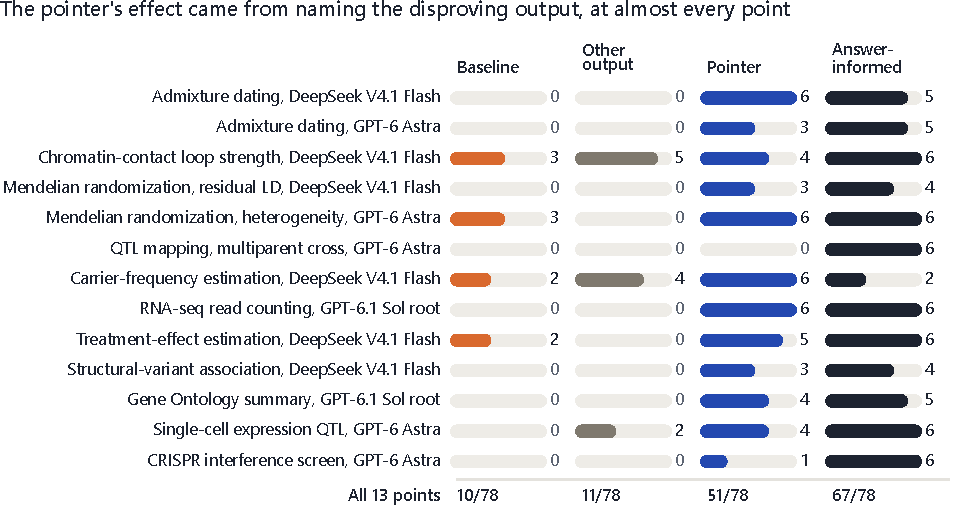
\includegraphics[width=\textwidth]{figures/fig8_points.pdf}
\caption{Replays at each of the 13 failure points: samples of 6 that followed up the disproving evidence under no note, the pointer to another output of the same
result, the pointer to the disproving output, and the answer-informed question. Rows name the problem and the model whose run produced the point. The read-counting
and Gene Ontology points are from BixBench3, the rest from GeneBench-Pro. All replies are by Claude Haiku 5.5.}
\label{fig:points}
\end{figure}

\subsection{In one model's plans, more structure produced unfalsifiable predictions}\label{sec:prereg}
In GPT-6.1 Sol's plans for one problem, the DamID reproduction, three plans per wording, no wording produced a prediction its result could contradict.
Asked for an observable expectation, it wrote structure: ``Four replicate profiles and two averaged profiles yield independently called target sets''.
Asked for a magnitude, it gave ranges of target genes spanning one to two orders of magnitude, called each ``deliberately broad'', and its result lay
inside both (\figref{fig:predictions}). Asked for a narrow prediction, it predicted only quantities fixed by the task, such as column counts.

When a prediction was returned beside the result, the comparison was lenient. With a prediction of hundreds of peaks and results of 1,605 to 1,747,
all three samples described the result as within or at the upper end of the prediction.

\begin{figure}[t]
\centering
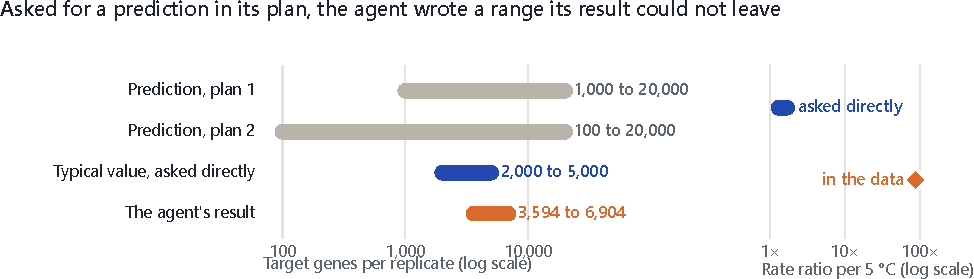
\includegraphics[width=\textwidth]{figures/fig9_predictions.pdf}
\caption{Left: target genes per replicate predicted by GPT-6.1 Sol in two plans for the DamID reproduction, the typical value it gives when asked directly, and its
result. Right: the rate ratio per 5\,$^\circ$C that GPT-6.1 Sol gives when asked directly, against the 87-fold jump in the reaction-kinetics data (our probe set).
Three plans or samples per wording.}
\label{fig:predictions}
\end{figure}

\subsection{Questions caused little rework on sound analyses; components that asserted a problem caused more}
Notes that asked or pointed seldom disturbed a sound analysis. Each question condition produced 0 of 18 samples of unwarranted rework at the
control points, and the pointer produced 1 of 18.

Components that asserted a problem did more harm. We tested three in replays on the original DeepSeek V4.1 Flash captures, at four control points
from passing runs. A fresh reader built on that model attached a note to 9 of 12 turns at those points. Most of its notes were the reader answering
the task itself, and at one point the agent then reopened settled work in 2 samples, against none without the reader.

A checker agent given the raw data and a passing answer argued that answer toward the value of a failing run, on 1 of the 2 sound analyses it
checked.

A referee that ran validity checks declared a violation in 7 of 15 checks on sound analyses over two rounds. Of those 7 violations, 4 named
properties the run had already handled. A question leaves the judgement with the agent, which holds the full context. A verdict from a component with less context
overrides it, and is wrong whenever that component is.

\subsection{Computed comparisons work; judged ones fail}
Every route that relied on the agent judging whether something mattered was lenient. Asked about the survey without the task, 10 of 10 samples
pointed at the wrong wave, the one with the largest drop. A correlation computed per wave exposes the reversed wave regardless of where suspicion
points.

Getting the agent to look is not enough either. Told to compute the per-chromosome ancestry table, Claude Haiku 5.5 did so in 10 of 10 forks
and kept the pooled answer in 10 of 10. One fork's reasoning called the spread ``real heterogeneity''. Treated as a hypothesis, heterogeneity
has a test on that table, and a relabelling test singles out one chromosome (\aref{app:relabel}).

\subsection{A fresh context is not an outside view}
A new context ran on the same defaults as the old one. A checker agent started from the raw data of the admixture problem, given the task and the
run's answer, printed the per-chromosome ancestry table and concluded that ``this scatter reflects real ancestry structure''. A fresh GPT-6.1 Sol call
given an agent's own account of its analysis named the step the agent had missed in 1 of 5 cases.

\section{Seven habits of a careful analyst}\label{sec:habits}

\tabref{tab:habits} states the habits whose absence the failures show. Each fires on an event in the agent's own work, specifies one act and a
condition for stopping, counters a behaviour of \sref{sec:behaviour}, and covers at least three unrelated cases in our data.

\begin{table}[t]
\centering\small
\footnotesize\caption{Seven habits of a careful analyst, derived from the traced failures. Cases: the unrelated analyses in our data where the habit would have applied.}
\label{tab:habits}
\begin{tabularx}{\textwidth}{@{}P{3.0cm}P{2.6cm}LP{2.6cm}P{1.9cm}P{2.3cm}@{}}
\toprule
Habit & Trigger & Act & Stop when & Counters & Cases\\
\midrule
1. Know why each field exists before using the data & a column records how, when or in which batch a row was made & use the field, or rule it out by its histogram; a median rules nothing out & the field is used or its distribution shows it inert & the familiar default & structural variants, carrier, CRISPR screen, load series (4)\\
2. Write the expected result before computing & a step is about to run & state a value or range the result could miss & the result is compared with it & no expectation & load series, kinetics, DamID, Mendelian randomization, read counting (5)\\
3. A check must be able to fail & an assumption is checked & split by the unit where the assumption could break & the check's result would differ were the assumption false & checks that cannot fail & survey, load series, admixture, QTL (4)\\
4. Your own disagreeing estimates are the result & two estimates of one quantity differ & explain the difference; report one value & the difference is attributed to a named choice or stratum & range reporting & carrier (two trials), treatment effect, structural variants, CRISPR screen (4)\\
5. ``Noise'', ``sparse'' and ``heterogeneity'' are claims & the agent is about to explain a discrepancy & compute what the explanation predicts & the prediction is tested & explaining it away & admixture, structural variants, Gene Ontology, carrier (4)\\
6. A nuisance that lines up with the effect is tested within itself & a technical variable tracks the variable of interest & test the effect within strata of the nuisance & the effect is measured within strata & the familiar default & single-cell eQTL, CRISPR screen, treatment effect (3)\\
7. Look at what a step removed or averaged away & a step filtered, masked or pooled data & inspect the removed or pooled part & its content is accounted for & checks in aggregate & read counting, QTL, admixture, load series (4)\\
\bottomrule
\end{tabularx}
\end{table}

The habits name practice that statistics and the experimental sciences have long taught. Examples are confirmation bias in hypothesis testing
\citep{wason1960}, batch effects aligned with the variable of interest \citep{leek2010}, and pooled associations that reverse within groups
\citep{simpson1951}. Their content was never the obstacle, because every model we asked could state it. Written into instructions, they did not
change the outcome (\sref{sec:steer}). In replay, what changed the agent's next step was a question or a pointer, at the reading turn, that named
the right output. Choosing that output is what no mechanism without the answer achieved.

For people building research agents, the results suggest five practices.
\begin{itemize}
\item Test a check by corrupting the data so that its assumption fails, and keep it only if its result changes.
\item Treat two disagreeing estimates of one quantity as a finding to explain, not a range to report.
\item Compute comparisons in the harness and report them to the agent as facts, instead of asking it to judge.
\item Prefer questions to verdicts from components that see less context than the agent.
\item Freeze an intervention before evaluating it, and evaluate it over many turns on held-out problems.
\end{itemize}

\section{Open problems}\label{sec:open}

\paragraph{1. Choosing the question without knowing the answer.} This is the measured bottleneck. The decisive question is taken up in 67 of
78 replayed samples, and the best question chosen without the answer reached 18 of 78. An output carries several real discrepancies, and every
reader we built selected one that was not the error.

\paragraph{2. Firing a habit at its trigger.} Each habit in \tabref{tab:habits} fires on an event the harness can observe: a result being read,
two estimates of the same quantity, a step that removed or averaged data, a column whose role is undeclared. Detecting these events across domains,
without a list written for one problem, is unsolved. Every condition in our replays arrived at the reading turn, so the effect of delivery at other
times is untested.

\paragraph{3. Defaults that leave no trace in the output.} A default applied without a test prints nothing that contradicts it. One candidate is
for the harness to re-run the agent's own analysis under a second, declared specification and report the difference as a fact. This is a proposal
we have not tested.

\paragraph{4. Training that rewards falsifying one's own result.} If the habit is absent because nothing rewards it, the remedy is a training signal
that does. That means episodes in which the reward depends on finding the flaw in one's own analysis, not on completing it.

\paragraph{5. Evaluating process interventions.} Benchmark convention is a large share of failure, 22 to 31\% here, and must be separated before a
score is read as analysis quality. Run-to-run variation is also large. Two DeepSeek V4.1 Flash trials on the same build each passed 2 of 10 problems,
but not the same two.

Single-turn replays measure uptake at one turn, and multi-turn forks can disagree with them. At the single-cell point, the agent followed up in no
single-turn replay and in 3 of 3 six-turn forks (\aref{app:multiturn}).

\section{Limitations and conclusion}\label{sec:limits}

\paragraph{Limitations.} The tasks are mostly genomics and genetics, with three constructed problems outside biology. All runs used one agent
harness, so harness and model effects are not separable. The steering results come from single-turn replays, in which Claude Haiku 5.5 answers in
another model's context without its private reasoning, at 13 points studied before the conditions were designed. The seven habits are derived from
the failures and have not been tested as interventions.

\paragraph{Conclusion.} The agents we studied had the knowledge their analyses needed and the evidence that their answers were wrong. What failed was
the choice of what to doubt, and nothing we built that lacked the answer could make that choice. That choice, made without the answer, is the open
problem.

\section*{Data and code availability}
The failure-replay method and data are at \url{https://github.com/shani-singh1/knowing-isnt-doing}. The repository holds per-sample outcomes for
every replay condition, the failure classification with the independent rating, the reasoning measurements, the condition, probe and criterion
texts, and the scripts that produce every figure, table and derived number. One script checks every number in this paper against those files.
Benchmark transcripts and captured model requests are not released, because they contain benchmark inputs and outputs.

\begin{thebibliography}{99}\setlength{\itemsep}{2pt}\small
\bibitem[Burns et~al.(2023)]{burns2023latent} Burns, C., Ye, H., Klein, D., and Steinhardt, J. (2023). Discovering latent knowledge in language
models without supervision. In \emph{ICLR}. \href{https://arxiv.org/abs/2212.03827}{arXiv:2212.03827}.
\bibitem[Cemri et~al.(2025)]{cemri2025mast} Cemri, M., et~al. (2025). Why do multi-agent LLM systems fail? In \emph{NeurIPS}.
\href{https://arxiv.org/abs/2503.13657}{arXiv:2503.13657}.
\bibitem[Chen et~al.(2025)]{chen2025scienceagentbench} Chen, Z., Chen, S., Ning, Y., et~al. (2025). ScienceAgentBench: Toward rigorous
assessment of language agents for data-driven scientific discovery. In \emph{ICLR}. \href{https://arxiv.org/abs/2410.05080}{arXiv:2410.05080}.
\bibitem[Gou et~al.(2024)]{gou2024critic} Gou, Z., Shao, Z., Gong, Y., Shen, Y., Yang, Y., Duan, N., and Chen, W. (2024). CRITIC: Large language
models can self-correct with tool-interactive critiquing. In \emph{ICLR}. \href{https://arxiv.org/abs/2305.11738}{arXiv:2305.11738}.
\bibitem[Huang et~al.(2024)]{huang2024selfcorrect} Huang, J., Chen, X., Mishra, S., Zheng, H.~S., Yu, A.~W., Song, X., and Zhou, D. (2024). Large
language models cannot self-correct reasoning yet. In \emph{ICLR}. \href{https://arxiv.org/abs/2310.01798}{arXiv:2310.01798}.
\bibitem[Huang et~al.(2025)]{huang2025biomni} Huang, K., et~al. (2025). Biomni: A general-purpose biomedical AI agent. bioRxiv.
\href{https://doi.org/10.1101/2025.05.30.656746}{doi:10.1101/2025.05.30.656746}.
\bibitem[Kadavath et~al.(2022)]{kadavath2022language} Kadavath, S., Conerly, T., Askell, A., et~al. (2022). Language models (mostly) know what
they know. \href{https://arxiv.org/abs/2207.05221}{arXiv:2207.05221}.
\bibitem[Koch et~al.(2026)]{koch2026bixbench3} Koch, Z., et~al. (2026). BixBench3: Benchmarking AI agents on research-study-scale computational
biology tasks. \href{https://arxiv.org/abs/2608.25286}{arXiv:2608.25286}.
\bibitem[Leek et~al.(2010)]{leek2010} Leek, J.~T., Scharpf, R.~B., Bravo, H.~C., et~al. (2010). Tackling the widespread and critical impact of
batch effects in high-throughput data. \emph{Nature Reviews Genetics}, 11(10):733--739. \href{https://doi.org/10.1038/nrg2825}{doi:10.1038/nrg2825}.
\bibitem[Lightman et~al.(2024)]{lightman2023verify} Lightman, H., et~al. (2024). Let's verify step by step. In \emph{ICLR}.
\href{https://arxiv.org/abs/2305.20050}{arXiv:2305.20050}.
\bibitem[Liu et~al.(2024)]{liu2024lost} Liu, N.~F., Lin, K., Hewitt, J., Paranjape, A., Bevilacqua, M., Petroni, F., and Liang, P. (2024). Lost in
the middle: How language models use long contexts. \emph{Transactions of the ACL}, 12:157--173.
\href{https://doi.org/10.1162/tacl_a_00638}{doi:10.1162/tacl\_a\_00638}.
\bibitem[Lu et~al.(2024)]{lu2024aiscientist} Lu, C., Lu, C., Lange, R.~T., Foerster, J., Clune, J., and Ha, D. (2024). The AI Scientist: Towards
fully automated open-ended scientific discovery. \href{https://arxiv.org/abs/2408.06292}{arXiv:2408.06292}.
\bibitem[Madaan et~al.(2023)]{madaan2023selfrefine} Madaan, A., Tandon, N., Gupta, P., et~al. (2023). Self-Refine: Iterative refinement with
self-feedback. In \emph{NeurIPS}. \href{https://arxiv.org/abs/2303.17651}{arXiv:2303.17651}.
\bibitem[Majumder et~al.(2025)]{majumder2025discoverybench} Majumder, B.~P., Surana, H., Agarwal, D., et~al. (2025). DiscoveryBench: Towards
data-driven discovery with large language models. In \emph{ICLR}. \href{https://arxiv.org/abs/2407.01725}{arXiv:2407.01725}.
\bibitem[Mitchener et~al.(2025)]{mitchener2025bixbench} Mitchener, L., Laurent, J.~M., et~al. (2025). BixBench: A comprehensive benchmark for
LLM-based agents in computational biology. \href{https://arxiv.org/abs/2503.00096}{arXiv:2503.00096}.
\bibitem[OpenAI(2026)]{openai2026genebench} OpenAI (2026). Introducing GeneBench-Pro. Public case-study package.
\url{https://openai.com/index/introducing-genebench-pro/}.
\bibitem[Orgad et~al.(2025)]{orgad2025know} Orgad, H., Toker, M., Gekhman, Z., Reichart, R., Szpektor, I., Kotek, H., and Belinkov, Y. (2025).
LLMs know more than they show: On the intrinsic representation of LLM hallucinations. In \emph{ICLR}.
\href{https://arxiv.org/abs/2410.02707}{arXiv:2410.02707}.
\bibitem[Shinn et~al.(2023)]{shinn2023reflexion} Shinn, N., et~al. (2023). Reflexion: Language agents with verbal reinforcement learning. In
\emph{NeurIPS}. \href{https://arxiv.org/abs/2303.11366}{arXiv:2303.11366}.
\bibitem[Simpson(1951)]{simpson1951} Simpson, E.~H. (1951). The interpretation of interaction in contingency tables. \emph{Journal of the Royal
Statistical Society B}, 13(2):238--241. \href{https://doi.org/10.1111/j.2517-6161.1951.tb00088.x}{doi:10.1111/j.2517-6161.1951.tb00088.x}.
\bibitem[Wason(1960)]{wason1960} Wason, P.~C. (1960). On the failure to eliminate hypotheses in a conceptual task. \emph{Quarterly Journal of
Experimental Psychology}, 12(3):129--140. \href{https://doi.org/10.1080/17470216008416717}{doi:10.1080/17470216008416717}.
\end{thebibliography}

\clearpage
\appendix
\renewcommand{\thetable}{A\arabic{table}}
\renewcommand{\thefigure}{A\arabic{figure}}
\setcounter{table}{0}
\setcounter{figure}{0}

\section{Models and settings}\label{app:models}
\begin{table}[H]
\centering\small
\caption{Models, model strings and settings. Neither the harness nor the replay code sets a sampling temperature, so each model ran at its provider's default.}
\label{tab:models}
\begin{tabularx}{\textwidth}{@{}P{3.8cm}P{4.0cm}L@{}}
\toprule
Role & Model string & Settings\\
\midrule
BixBench3 root agent & \texttt{openai/gpt-6.1-sol} & reasoning effort maximum\\
BixBench3 delegated execution & DeepSeek V4.1 Flash & effort not recorded\\
GeneBench-Pro agent, two trials & \texttt{deepseek/deepseek-v4.1-flash} & reasoning effort maximum\\
GeneBench-Pro agent, one trial & \texttt{openai/gpt-6-astra} & reasoning effort maximum; some steps delegated to DeepSeek V4.1 Flash\\
Live runs and every replay & \texttt{claude-haiku-5-5} & effort high, adaptive thinking with summarised display, output limit 64,000 tokens in replays; maximum effort where stated\\
Judge; classification rater; one comparison & \texttt{claude-sonnet-5-5} & judge: effort low, the reply's text and code only; rater: effort high, adaptive thinking; comparison: effort high\\
Second judge & \texttt{claude-opus-5-5} & effort low, the same prompt as the judge\\
Knowledge probes & as named in \figref{fig:know} & effort high (Claude); the agent's own settings (GPT-6.1 Sol)\\
\bottomrule
\end{tabularx}
\end{table}

\section{Conditions}\label{app:conditions}
\begin{table}[H]
\centering\small
\caption{Replay conditions. Notes are appended after the last tool result as a bracketed system line. Reader questions are generated per sample by a
separate Claude Haiku 5.5 call and delivered as ``A reviewer who read only the task and your last output asks: \ldots''. A reader that answers NONE adds
nothing.}
\label{tab:conditions}
\begin{tabularx}{\textwidth}{@{}P{3.6cm}L@{}}
\toprule
Condition & What changes\\
\midrule
No note (baseline) & nothing; reasoning effort high\\
Maximum reasoning effort & effort maximum, output limit 64,000 tokens\\
Generic reminder & ``Before you continue: is there anything in what you have computed so far that you have not yet accounted for?''\\
Self-review prompt & ``Before you continue: what is the one question a careful reviewer would ask about the output you just got, before letting you build on it? Ask it, then answer it from the data.''\\
Fresh reader: open question & a separate call sees the task, the last code and its output, and asks the single most important question before building on it\\
Fresh reader: assumptions & a separate call sees the task, all code and the last output, lists what the analysis takes as given, and asks for the observation that would show the likeliest false and consequential assumption is false\\
Fresh reader: largest impact & a separate call collects evidence in the output that disagrees with the analysis and asks about the item that would change the answer most\\
Fresh reader: disagreements & a separate call looks only for disagreement printed in the output (two estimates of one quantity, a misfit diagnostic, failing units, a part that disagrees with the rest)\\
Fresh readers: all questions & the questions of the assumptions, largest-impact and disagreements readers, as one numbered list\\
Pointer to another output & the pointer's wording, naming another output printed in the same tool result, not the disproving one\\
Pointer to the output & ``Before you continue, look again at \emph{label} in the output you just got'', where \emph{label} is the agent's own printed label for the disproving output\\
Answer-informed question & the question an analyst who knew the error would ask, written from the tracing\\
\bottomrule
\end{tabularx}
\end{table}
At the control points, where there is no disproving output, the pointer names the output carrying the result the agent is about to build on, and the pointer to
another output names a secondary diagnostic printed in the same result. Both pointer conditions, and their labels, were written down before they were run.

\section{Follow-up criteria}\label{app:criteria}
Fixed before any replay. Admixture dating: compares the ancestry fraction per haplotype per chromosome, or questions whether labels are consistent across
chromosomes. Chromatin-contact loop strength: investigates the case-only block of high pixels or the relation of coverage to GC content, or excludes the block
from the background model. Mendelian randomization, residual correlation: treats the permutation result as a sign that the instrument model is wrong.
Mendelian randomization, heterogeneity: treats $Q$ as evidence that the model is wrong and finds which instruments drive it. QTL mapping: computes held-out
concordance per marker. Carrier frequency: names both estimates and works out which is right. Read counting: asks which loci have no counts and why. Treatment
effect: asks why adjusting for the covariate moves the estimate. Structural-variant association: asks why the adjustment moves the estimate. Gene Ontology
summary: treats the root-only genes as a possible defect in its own lookup and tests it. Single-cell expression QTL: tests contamination by genotype beyond an
additive term. CRISPR interference screen: tests dependence on GC content beyond a linear term, or by plate, among the guides where GC tracks knockdown. Control
points: a reply is unwarranted rework when its only content re-checks a settled quantity or when it abandons a sound approach on a weak signal.

\section{Per-point replay counts}\label{app:points}
\begin{table}[H]
\centering\scriptsize
\caption{Replays: samples of 6 that followed up, per failure point and condition (columns in the order of \tabref{tab:conditions}); last row, unwarranted rework
at the control points, where the answer-informed question is not defined.}
\label{tab:points}
\setlength{\tabcolsep}{3pt}
\begin{tabularx}{\textwidth}{@{}L*{12}{c}@{}}
\toprule
Failure point & Base & Max & Gen. & Self & Open & Assm. & Imp. & All & Dis. & Other & Ptr. & Ans.\\
\midrule
\inputrows{figures/tab_points.tex}
\bottomrule
\end{tabularx}
\end{table}
At the carrier point, replies to a note that stated the two estimates often referred to ``the two numbers'' without restating them. The judge, which does not
see the note, scored several such replies as not naming the estimates. The criterion fixed before the replays requires the reply to name both estimates, so the
scores above stand. As a sensitivity result, every condition at that point was re-scored by the same judge with the same criterion, shown the note the agent had
received (\tabref{tab:sens}). The largest change is the disagreement reader, whose question named both estimates: 0 to 6 of 6 at the point, 18 to 24 of 78 overall.
No conclusion in the paper changes.
\begin{table}[H]
\centering\small
\caption{Sensitivity scoring at the carrier failure point (replays): samples of 6 that followed up, as scored and with the note visible to the
judge, and the pooled count over the 13 points under each.}
\label{tab:sens}
\begin{tabular}{@{}lcccc@{}}
\toprule
Condition & Carrier, scored & Carrier, note visible & All points, scored & All points, note visible\\
\midrule
\inputrows{figures/tab_sensitivity.tex}
\bottomrule
\end{tabular}
\end{table}

\section{Paired comparisons}\label{app:tests}
Replays at the 13 failure points. For each pair of conditions: the points where the first had more follow-ups than the second, fewer, and the
same; an exact two-sided sign test on the points that differ; and an exact sign-flip permutation test on the per-point differences. Pooled rates
carry 95\% intervals from a bootstrap over points (20,000 draws), drawn in \figref{fig:steering}; with 13 points they are approximate. The
comparisons are not corrected for multiplicity, and no claim rests on one of them alone. With 0 events in 18 samples, the two-sided 95\% upper
bound on a rate is 18\%.
\begin{table}[H]
\centering\small
\caption{Paired per-point comparisons (replays, 13 failure points, 6 samples per point and condition).}
\label{tab:tests}
\begin{tabular}{@{}llccccc@{}}
\toprule
Condition & Against & Above & Below & Tied & Sign $p$ & Permutation $p$\\
\midrule
\inputrows{figures/tab_tests.tex}
\bottomrule
\end{tabular}
\end{table}

\section{Classification and all cause groups}\label{app:groups}
A cause is \emph{established} when the tracing report established it and named one class (56 failures), and \emph{probable} otherwise (48). For 16 failures
the report names two causes of equal weight; the primary classification takes the first-listed one, and the released data give the other. The independent
rater agreed with the primary classification on 55 of 58 GeneBench-Pro keys ($\kappa = 0.93$) and on 33 of 46 BixBench3 outputs ($\kappa = 0.54$). Of the 13
BixBench3 disagreements, 9 involve the class for task wording and reference convention. Over the 31 cause groups attributable to the agent under the primary
classification, the default, aggregate and on-screen classes hold 58\%, 19\% and 23\%.

\begin{small}
\setlength{\tabcolsep}{4pt}
\begin{longtable}{@{}>{\raggedright\arraybackslash}p{4.0cm}>{\raggedright\arraybackslash}p{4.0cm}c>{\raggedright\arraybackslash}p{1.7cm}>{\raggedright\arraybackslash}p{2.8cm}c@{}}
\caption{Every cause group: the failures from one run of one problem that share a primary class, with the independent rater's classes for the same failures and the number
of established causes.}\label{tab:groups}\\
\toprule
Problem & Run & Failures & Primary class & Independent rater & Established\\
\midrule\endfirsthead
\toprule
Problem & Run & Failures & Primary class & Independent rater & Established\\
\midrule\endhead
\inputrows{figures/tab_groups.tex}
\bottomrule
\end{longtable}
\end{small}

\section{Interventions designed and tested}\label{app:history}
We designed 49 interventions and tested 46, in two phases: 25 replayed on the original DeepSeek V4.1 Flash, GPT-6 Astra and GPT-6.1 Sol requests
and 24 replayed with Claude Haiku 5.5. \tabref{tab:history} groups them by kind; wording variants of one idea
count as one intervention.
\begin{small}
\begin{longtable}{@{}>{\raggedright\arraybackslash}p{5.2cm}>{\raggedright\arraybackslash}p{10.6cm}@{}}
\caption{Interventions by kind, with the result that decided each. Counts are replays unless stated.}\label{tab:history}\\
\toprule
Intervention & Result\\
\midrule\endfirsthead
\toprule
Intervention & Result\\
\midrule\endhead
Notes at turn boundaries (plan saved, step done, before finishing; generic completion notes) & no change in what the agent checked; a note before the final step was ignored in 6 of 6 samples\\
Plan fields asking for expected results (six wordings) & form of the plan changed, content never falsifiable (\sref{sec:prereg})\\
A note at the start of a step, with the agent's own prediction returned beside its result & the named check computed in 5 of 6 and 6 of 6, on one problem (\aref{app:multiturn}); the comparison with the prediction lenient\\
Notes at the step where an assumption is used (identification, per-part completion) & per-part values computed in 6 of 6 samples, none split by the unit that mattered\\
Rewritten or removed instructions to work economically & first step changed (9 to 17 of 30), graded outcome unchanged (1 of 15); acting on the on-screen number 1 of 15 against 3 of 15\\
Fresh readers (eight versions on the original captures; four and their combination on Claude) & 10 to 18 of 78 on Claude; on the original captures, notes on 9 of 12 sound turns\\
A checker agent with the raw data; a referee running validity checks & checker argued a passing answer toward a failing run's value; referee flagged 4 of 8 and 3 of 7 checks on sound analyses\\
A fresh agent restarted with a prior analyst's answer; a fresh model given the agent's account & the restarted agent reproduced the prior answer; the fresh model named the missed step in 1 of 5 cases\\
Reasoning effort: maximum, extra-high, by turn, re-asking an ending turn at maximum & load series 1 to 15 of 15 by schedule; 9 of 78 against 10 of 78 at the failure points\\
A stronger model (Claude Sonnet 5.5) & load series 9 of 10\\
Generic reminder; self-review prompt & 11 of 78 each\\
List of expert checks at the first look at the data & named the decisive check for 4 of 9 problems; forks 9 of 16 against 9 of 18 (\aref{app:multiturn})\\
Every reader's question at once (one turn; six turns) & 15 of 78; six-turn forks 8 of 12 against 5 of 12\\
Pointer to the disproving output; to another output & 51 of 78; 11 of 78\\
Answer-informed question & 67 of 78\\
Not tested: a reader that inspects code choices; a live comparison of a design against the baseline; tests of the seven habits & designed only\\
\bottomrule
\end{longtable}
\end{small}

\section{Tasks}\label{app:tasks}
\textbf{BixBench3} \citep{koch2026bixbench3}, 13 tasks with a graded run (identifier: analysis). Task 1 (10.1101/2025.06.17.659900): DamID target calling
and bulk RNA-seq in \emph{C. elegans}. Task 2 (10.64898/2026.02.11.704850): mouse bulk RNA-seq, differential expression, GO enrichment and
ligand--receptor scores. Task 4 (10.64898/2026.02.03.703548): de novo transcriptome assembly and ddRAD population genomics. Task 8
(10.1038/s42003-022-03654-9): xenograft and tumorsphere RNA-seq with gene-set enrichment. Task 10 (10.1038/s41467-023-44243-6): transcript-level
counts and differential expression. Task 12 (10.1101/2025.06.02.657493): bacterial RNA-seq time course, read counting and differential expression.
Task 13 (10.64898/2026.03.10.709901): single-cell microsatellite lineage tracing. Task 14 (10.1101/2025.07.21.665972): mRNA and miRNA differential
expression. Task 15 (10.64898/2026.01.09.698641): differential expression, splicing and long-read transcript counts. Task 16
(10.1101/2025.07.31.667834): antifungal RNA-seq in two \emph{Candida glabrata} strains with GO Slim summaries. Task 18 (10.64898/2026.01.02.697332):
RNA-seq and ATAC-seq differential analysis. Task 19 (10.64898/2026.01.31.702960): mRNA and small-RNA analysis in \emph{C. elegans} mutants. Task 20
(10.64898/2026.02.04.703711): 16S community composition, taxon productivity and a null interaction simulation. Tasks 3, 5, 6, 9 and 11 were run only
after the tracing began, task 7 was stopped by a spending limit before grading, and task 17 was not run.

\textbf{GeneBench-Pro} \citep{openai2026genebench} public case studies, 10 problems (identifier: analysis):

\noindent{\small\begin{tabularx}{\textwidth}{@{}P{7.4cm}L@{}}
\texttt{popgen\_recent\_pulse\_sexbias} & admixture dating\\
\texttt{multiparent\_qtl\_hmm\_lmm} & QTL mapping, multiparent cross\\
\texttt{hic\_sv\_masked\_loop\_strength} & chromatin-contact loop strength\\
\texttt{statgen\_cis\_mvmr\_winnerscurse\_scaling\_ldaware} & Mendelian randomization\\
\texttt{statgen\_scrna\_ambient\_state\_eqtl} & single-cell expression QTL\\
\texttt{crispri\_casrx\_transcript\_vs\_locus} & CRISPR interference screen\\
\texttt{structural\_inversion\_subhap\_expression\_risk} & structural-variant association\\
\texttt{carrier\_cnv\_pseudogene\_residual\_risk} & carrier frequency\\
\texttt{txr1\_mtb\_causal\_sv} & treatment effect\\
\texttt{wf\_selection} & selection inference\\
\end{tabularx}}
The control points come from passing runs of the selection-inference problem (two) and the single-cell problem (one).

\textbf{Our probe set}: an electrical-load series, a four-wave survey and a reaction-kinetics series, used for the knowledge probes and the
reasoning-effort study only.

\section{Confound audit}\label{app:confounds}
Before any replay we checked, and where needed corrected, the following classes of harness effect: limits on model output length, including whether reasoning
tokens count against them; prompt-cache behaviour and token accounting; whether reasoning content is carried between turns; instructions in the system prompt or
in delegation briefs that discourage additional analysis; whether a failed or interrupted code cell is reported to the agent; and how evaluation matches delivered
files to required outputs.

\section{Task wording and reference convention}\label{app:conventions}
Examples, without answer values. BixBench3 task 12: the task instructs that reads mapping to multiple genomic locations are not counted; the reference counts at
multi-copy loci are consistent with such reads having been counted. BixBench3 task 10: the output universe follows an annotation release; the task names no release,
and the reference corresponds to an earlier release than the one retrieved at run time. GeneBench-Pro structural-variant association: equally defensible constructions
of the dosage variable give estimates spread over a range wider than the grading tolerance. GeneBench-Pro chromatin-contact loop strength: the control estimate varies
across defensible specifications of the expected background by more than the tolerance.

\section{Multi-turn and early forks}\label{app:multiturn}
\textbf{Six-turn forks.} From four failure points, three forks per arm, each fork was continued for six turns and judged on whether any turn followed up
(\figref{fig:multiturn}, left).

\textbf{An early list of checks.} A separate model call that saw the task and the first look at the data listed up to five checks an expert would run. The list
named the decisive check for only 4 of 9 GeneBench-Pro problems. Forks given the list and continued to the end passed 9 of 16, against 9 of 18 without it, with two
forks per arm and one arm that failed to run (\figref{fig:multiturn}, right). With so few forks on the problems where the list named the check, this comparison does
not separate early delivery from the content of the list.

\textbf{A note at the start of a step.} On one problem, the DamID reproduction, a note at the start of a step with the agent's own prediction returned beside the
step's result got the named check computed in 5 of 6 and 6 of 6 samples in two rounds. The comparison with the prediction was lenient (\sref{sec:prereg}).

\begin{figure}[H]
\centering
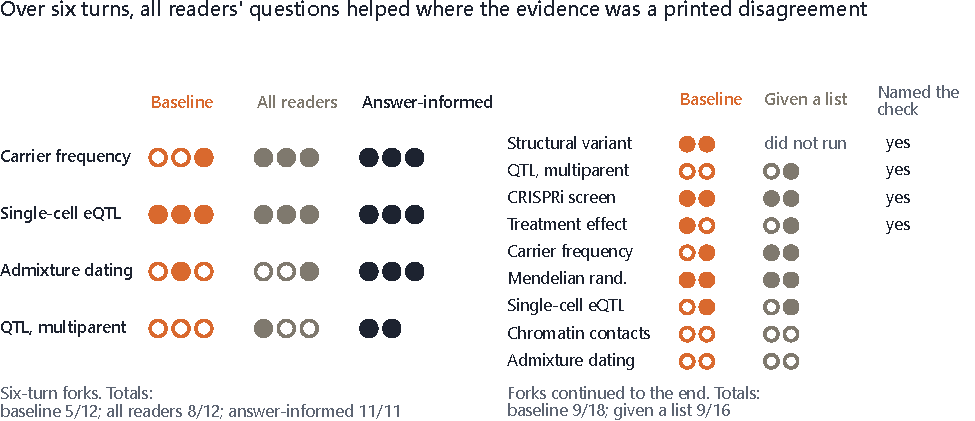
\includegraphics[width=\textwidth]{figures/figA1_multiturn.pdf}
\caption{Left: six-turn forks from four failure points, three per arm (two for one answer-informed arm), judged on whether any turn followed up. Right: GeneBench-Pro
forks from the first look at the data in nine problems, two per arm, continued to the end, with and without a list of up to five checks written by a separate call that
saw only the task and the data so far; one arm with the list failed to run. All forks by Claude Haiku 5.5.}
\label{fig:multiturn}
\end{figure}

\section{The relabelling test on the admixture table}\label{app:relabel}
Claude Haiku 5.5, told to compute the per-chromosome ancestry fractions, printed them for each of two haplotypes on four chromosomes. If the ancestry labels are
inverted on one chromosome, relabelling that chromosome (each fraction $x$ becomes $1-x$) should reduce the spread across chromosomes in both haplotypes at once.
Under sampling noise no single relabelling should stand out. Of the four single-chromosome relabellings of the printed table, only that of the third chromosome
reduces the summed standard deviation across chromosomes, from 0.641 to 0.403; the others leave it at 0.55 or above. With four units the test is weak, but it is one
computation on a table the agent had already printed.

\end{document}
